\chapter{Introduction}
Fuzzy logic (FL) and genetic algorithms are members of a family of so-called soft computing methods along with
neural nets (NN) and probabilistic reasoning\cite{cordon:01bk}. Each of these methods has particular strengths
in specific domains, but all are employed in application which require computation based on imprecise, vague,
or uncertain data. In recent years, NNs have risen greatly in popularity as improvements in compute power and
algorithm development have allowed their application to a wide variety of problems via their role in dep
learning\cite{Goodfellow-et-al-2016}. While FL has seen much less application in deep learning applications,
it has long been shown to be particularly useful in feedback control applications of nonlinear
systems\cite{MAMDANI19751}. FL excels at encoding expert knowlede of a human operator in machine-interpretable
logic. In many cases, however, it is difficult or impossible to encode a knowledge base which is sufficient to
control a system satisfactorily by hand; in these cases, a GA may be applied to tune or even learn a FL system
to accomplish the task.

\section{Fuzzy Logic}
The basic component of a FL system consists of fuzzy membership sets\cite{ZADEH1965338}, which are an
extension of classical binary set theory. The advantage of fuzzy set theory is that an element may share
membership across many sets simultaneously in contrast to traiditonal set logic (see
\crefrange{f:crispsets}{f:fuzzysets}). This formal encapsulation of ``fuzziness'' provides a method for
machine instructions to operate on imprecise values. Fuzzy sets constitute the most basic element of a FL
system; they are made useful in controls application when combined with a rule base (RB).

\begin{figure}[ht]
    \centering
    \begin{tikzpicture}[gnuplot]
%% generated with GNUPLOT 5.0p3 (Lua 5.1; terminal rev. 99, script rev. 100)
%% Thu 29 Mar 2018 12:26:43 AM EDT
\gpmonochromelines
\path (0.000,0.000) rectangle (12.500,8.750);
\gpcolor{color=gp lt color border}
\gpsetlinetype{gp lt border}
\gpsetdashtype{gp dt solid}
\gpsetlinewidth{1.00}
\draw[gp path] (1.320,1.601)--(1.500,1.601);
\draw[gp path] (11.947,1.601)--(11.767,1.601);
\node[gp node right] at (1.136,1.601) {$0$};
\draw[gp path] (1.320,2.834)--(1.500,2.834);
\draw[gp path] (11.947,2.834)--(11.767,2.834);
\node[gp node right] at (1.136,2.834) {$0.2$};
\draw[gp path] (1.320,4.067)--(1.500,4.067);
\draw[gp path] (11.947,4.067)--(11.767,4.067);
\node[gp node right] at (1.136,4.067) {$0.4$};
\draw[gp path] (1.320,5.299)--(1.500,5.299);
\draw[gp path] (11.947,5.299)--(11.767,5.299);
\node[gp node right] at (1.136,5.299) {$0.6$};
\draw[gp path] (1.320,6.532)--(1.500,6.532);
\draw[gp path] (11.947,6.532)--(11.767,6.532);
\node[gp node right] at (1.136,6.532) {$0.8$};
\draw[gp path] (1.320,7.765)--(1.500,7.765);
\draw[gp path] (11.947,7.765)--(11.767,7.765);
\node[gp node right] at (1.136,7.765) {$1$};
\draw[gp path] (1.320,0.985)--(1.320,1.165);
\draw[gp path] (1.320,8.381)--(1.320,8.201);
\node[gp node center] at (1.320,0.677) {$50$};
\draw[gp path] (3.091,0.985)--(3.091,1.165);
\draw[gp path] (3.091,8.381)--(3.091,8.201);
\node[gp node center] at (3.091,0.677) {$55$};
\draw[gp path] (4.862,0.985)--(4.862,1.165);
\draw[gp path] (4.862,8.381)--(4.862,8.201);
\node[gp node center] at (4.862,0.677) {$60$};
\draw[gp path] (6.634,0.985)--(6.634,1.165);
\draw[gp path] (6.634,8.381)--(6.634,8.201);
\node[gp node center] at (6.634,0.677) {$65$};
\draw[gp path] (8.405,0.985)--(8.405,1.165);
\draw[gp path] (8.405,8.381)--(8.405,8.201);
\node[gp node center] at (8.405,0.677) {$70$};
\draw[gp path] (10.176,0.985)--(10.176,1.165);
\draw[gp path] (10.176,8.381)--(10.176,8.201);
\node[gp node center] at (10.176,0.677) {$75$};
\draw[gp path] (11.947,0.985)--(11.947,1.165);
\draw[gp path] (11.947,8.381)--(11.947,8.201);
\node[gp node center] at (11.947,0.677) {$80$};
\draw[gp path] (1.320,8.381)--(1.320,0.985)--(11.947,0.985)--(11.947,8.381)--cycle;
\node[gp node center,rotate=-270] at (0.246,4.683) {$\mu$, Membership value};
\node[gp node center] at (6.633,0.215) {Temperature, $\deg$};
\draw[gp path] (8.915,4.221)--(8.915,5.145)--(11.763,5.145)--(11.763,4.221)--cycle;
\gpfill{color=gp lt color border,gp pattern 0,pattern color=.} (1.320,7.765)--(4.862,7.765)--(4.862,1.601)--(8.405,1.601)%
    --(8.405,1.601)--(11.947,1.601)--(11.947,1.601)--cycle;
\draw[gp path] (1.320,7.765)--(4.862,7.765)--(4.862,1.601)--(8.405,1.601)--(11.947,1.601);
\gpfill{color=gp lt color border,gp pattern 1,pattern color=.} (1.320,1.601)--(4.862,1.601)--(4.862,7.765)--(8.405,7.765)%
    --(8.405,1.601)--(11.947,1.601)--(11.947,1.601)--cycle;
\gpsetdashtype{gp dt 2}
\draw[gp path] (1.320,1.601)--(4.862,1.601)--(4.862,7.765)--(8.405,7.765)--(8.405,1.601)%
  --(11.947,1.601);
\gpfill{color=gp lt color border,opacity=0.25} (1.320,1.601)--(4.862,1.601)--(4.862,1.601)--(8.405,1.601)%
    --(8.405,7.765)--(11.947,7.765)--(11.947,1.601)--cycle;
\gpsetdashtype{gp dt 3}
\draw[gp path] (1.320,1.601)--(4.862,1.601)--(8.405,1.601)--(8.405,7.765)--(11.947,7.765)%
  --(11.947,1.601);
\gpfill{color=gpbgfillcolor} (8.915,4.221)--(11.763,4.221)--(11.763,5.145)--(8.915,5.145)--cycle;
\gpsetdashtype{gp dt solid}
\draw[gp path] (8.915,4.221)--(8.915,5.145)--(11.763,5.145)--(11.763,4.221)--cycle;
\node[gp node right] at (10.479,4.991) {Cool};
\gpfill{color=gp lt color border,gp pattern 0,pattern color=.} (10.663,4.914)--(11.579,4.914)--(11.579,5.068)--(10.663,5.068)--cycle;
\draw[gp path] (10.663,4.914)--(11.579,4.914)--(11.579,5.068)--(10.663,5.068)--cycle;
\node[gp node right] at (10.479,4.683) {Warm};
\gpfill{color=gp lt color border,gp pattern 1,pattern color=.} (10.663,4.606)--(11.579,4.606)--(11.579,4.760)--(10.663,4.760)--cycle;
\gpsetdashtype{gp dt 2}
\draw[gp path] (10.663,4.606)--(11.579,4.606)--(11.579,4.760)--(10.663,4.760)--cycle;
\node[gp node right] at (10.479,4.375) {Hot};
\gpfill{color=gp lt color border,opacity=0.25} (10.663,4.298)--(11.579,4.298)--(11.579,4.452)--(10.663,4.452)--cycle;
\gpsetdashtype{gp dt 3}
\draw[gp path] (10.663,4.298)--(11.579,4.298)--(11.579,4.452)--(10.663,4.452)--cycle;
\gpsetdashtype{gp dt solid}
\draw[gp path] (1.320,8.381)--(1.320,0.985)--(11.947,0.985)--(11.947,8.381)--cycle;
%% coordinates of the plot area
\gpdefrectangularnode{gp plot 1}{\pgfpoint{1.320cm}{0.985cm}}{\pgfpoint{11.947cm}{8.381cm}}
\end{tikzpicture}
%% gnuplot variables

    \caption{Crisp (classical) logic set transitions are discrete and abrupt}\label{f:crispsets}
\end{figure}

\begin{figure}[ht]
    \centering
    \begin{tikzpicture}[gnuplot]
%% generated with GNUPLOT 5.0p3 (Lua 5.1; terminal rev. 99, script rev. 100)
%% Thu 29 Mar 2018 12:26:43 AM EDT
\gpmonochromelines
\path (0.000,0.000) rectangle (12.500,8.750);
\gpcolor{color=gp lt color border}
\gpsetlinetype{gp lt border}
\gpsetdashtype{gp dt solid}
\gpsetlinewidth{1.00}
\draw[gp path] (1.320,1.601)--(1.500,1.601);
\draw[gp path] (11.947,1.601)--(11.767,1.601);
\node[gp node right] at (1.136,1.601) {$0$};
\draw[gp path] (1.320,2.834)--(1.500,2.834);
\draw[gp path] (11.947,2.834)--(11.767,2.834);
\node[gp node right] at (1.136,2.834) {$0.2$};
\draw[gp path] (1.320,4.067)--(1.500,4.067);
\draw[gp path] (11.947,4.067)--(11.767,4.067);
\node[gp node right] at (1.136,4.067) {$0.4$};
\draw[gp path] (1.320,5.299)--(1.500,5.299);
\draw[gp path] (11.947,5.299)--(11.767,5.299);
\node[gp node right] at (1.136,5.299) {$0.6$};
\draw[gp path] (1.320,6.532)--(1.500,6.532);
\draw[gp path] (11.947,6.532)--(11.767,6.532);
\node[gp node right] at (1.136,6.532) {$0.8$};
\draw[gp path] (1.320,7.765)--(1.500,7.765);
\draw[gp path] (11.947,7.765)--(11.767,7.765);
\node[gp node right] at (1.136,7.765) {$1$};
\draw[gp path] (1.320,0.985)--(1.320,1.165);
\draw[gp path] (1.320,8.381)--(1.320,8.201);
\node[gp node center] at (1.320,0.677) {$50$};
\draw[gp path] (3.091,0.985)--(3.091,1.165);
\draw[gp path] (3.091,8.381)--(3.091,8.201);
\node[gp node center] at (3.091,0.677) {$55$};
\draw[gp path] (4.862,0.985)--(4.862,1.165);
\draw[gp path] (4.862,8.381)--(4.862,8.201);
\node[gp node center] at (4.862,0.677) {$60$};
\draw[gp path] (6.634,0.985)--(6.634,1.165);
\draw[gp path] (6.634,8.381)--(6.634,8.201);
\node[gp node center] at (6.634,0.677) {$65$};
\draw[gp path] (8.405,0.985)--(8.405,1.165);
\draw[gp path] (8.405,8.381)--(8.405,8.201);
\node[gp node center] at (8.405,0.677) {$70$};
\draw[gp path] (10.176,0.985)--(10.176,1.165);
\draw[gp path] (10.176,8.381)--(10.176,8.201);
\node[gp node center] at (10.176,0.677) {$75$};
\draw[gp path] (11.947,0.985)--(11.947,1.165);
\draw[gp path] (11.947,8.381)--(11.947,8.201);
\node[gp node center] at (11.947,0.677) {$80$};
\draw[gp path] (1.320,8.381)--(1.320,0.985)--(11.947,0.985)--(11.947,8.381)--cycle;
\node[gp node center,rotate=-270] at (0.246,4.683) {$\mu$, Membership value};
\node[gp node center] at (6.633,0.215) {Temperature, $\deg$};
\draw[gp path] (8.915,4.221)--(8.915,5.145)--(11.763,5.145)--(11.763,4.221)--cycle;
\gpfill{color=gp lt color border,gp pattern 0,pattern color=.} (1.320,7.765)--(3.091,7.765)--(6.634,1.601)--(10.176,1.601)%
    --(11.947,1.601)--(11.947,1.601)--cycle;
\draw[gp path] (1.320,7.765)--(3.091,7.765)--(6.634,1.601)--(10.176,1.601)--(11.947,1.601);
\gpfill{color=gp lt color border,gp pattern 1,pattern color=.} (1.320,1.601)--(3.091,1.601)--(6.634,7.765)--(10.176,1.601)%
    --(11.947,1.601)--(11.947,1.601)--cycle;
\gpsetdashtype{gp dt 2}
\draw[gp path] (1.320,1.601)--(3.091,1.601)--(6.634,7.765)--(10.176,1.601)--(11.947,1.601);
\gpfill{color=gp lt color border,opacity=0.25} (1.320,1.601)--(3.091,1.601)--(6.634,1.601)--(10.176,7.765)%
    --(11.947,7.765)--(11.947,1.601)--cycle;
\gpsetdashtype{gp dt 3}
\draw[gp path] (1.320,1.601)--(3.091,1.601)--(6.634,1.601)--(10.176,7.765)--(11.947,7.765)%
  --(11.947,1.601);
\gpfill{color=gpbgfillcolor} (8.915,4.221)--(11.763,4.221)--(11.763,5.145)--(8.915,5.145)--cycle;
\gpsetdashtype{gp dt solid}
\draw[gp path] (8.915,4.221)--(8.915,5.145)--(11.763,5.145)--(11.763,4.221)--cycle;
\node[gp node right] at (10.479,4.991) {Cool};
\gpfill{color=gp lt color border,gp pattern 0,pattern color=.} (10.663,4.914)--(11.579,4.914)--(11.579,5.068)--(10.663,5.068)--cycle;
\draw[gp path] (10.663,4.914)--(11.579,4.914)--(11.579,5.068)--(10.663,5.068)--cycle;
\node[gp node right] at (10.479,4.683) {Warm};
\gpfill{color=gp lt color border,gp pattern 1,pattern color=.} (10.663,4.606)--(11.579,4.606)--(11.579,4.760)--(10.663,4.760)--cycle;
\gpsetdashtype{gp dt 2}
\draw[gp path] (10.663,4.606)--(11.579,4.606)--(11.579,4.760)--(10.663,4.760)--cycle;
\node[gp node right] at (10.479,4.375) {Hot};
\gpfill{color=gp lt color border,opacity=0.25} (10.663,4.298)--(11.579,4.298)--(11.579,4.452)--(10.663,4.452)--cycle;
\gpsetdashtype{gp dt 3}
\draw[gp path] (10.663,4.298)--(11.579,4.298)--(11.579,4.452)--(10.663,4.452)--cycle;
\gpsetdashtype{gp dt solid}
\draw[gp path] (1.320,8.381)--(1.320,0.985)--(11.947,0.985)--(11.947,8.381)--cycle;
%% coordinates of the plot area
\gpdefrectangularnode{gp plot 1}{\pgfpoint{1.320cm}{0.985cm}}{\pgfpoint{11.947cm}{8.381cm}}
\end{tikzpicture}
%% gnuplot variables

    \caption{Fuzzy sets allow for multiple membership, so a value can smoothly transition from being a member
    of set to another.}\label{f:fuzzysets}
\end{figure}

A fuzzy inference system (FIS) is a control system built on the basic principles of fuzzy
logic\cite{kosko:91bk}\cite{kosko:93sciam}. It can take an arbitrary number analog inputs and map them to a
set of logical variables ranging from 0 to 1. This mapping is performed by membership functions (MF), which
determine the degree of membership each input has to a function. Each input typically has multiple Mfs,
allowing the input value (a so-called ``crisp value'' to be given membership in multiple sets
simultaneously. The memberships are used to make an inference about the input according to linguistic rules.
The RB is composed of IF-THEN statements which determine the crisp output variable. For example, if the
membership sets in \cref{f:fuzzysets} were to be the input to a fan controller, and the output membership
functions were as they are in \cref{f:outputfan}, the rules could be described as:

\vspace{2em}
\begin{tabular}{cccccc}
        IF &  \emph{temperature} is & COOL, & THEN & \emph{fan speed} is & OFF\\
        IF &  \emph{temperature} is & WARM, & THEN & \emph{fan speed} is & LOW\\
        IF &  \emph{temperature} is & HOT,  & THEN & \emph{fan speed} is & HIGH
\end{tabular}
\vspace{2em}

These rules can be succintly placed in a table as shown in \cref{t:fanspeed}. This representation becomes more
useful still another input is addded to the controller. By using the set of rules and the MFs, the FIS is able
to determine an appropriate crisp output given a set of crisp inputs. The FIS representation is in essence a
transfer function, but a transfer function which can be arbitrarily complex. The common representation of a
FIS shown in \cref{f:fis_block} shows the components of a FIS.

\begin{table}[ht]
    \centering
    \caption{Example rule base for a fictitious fan speed controller}\label{t:fanspeed}
    \begin{tabular}{c|c|c|c}
        Temperature & Cool & Warm & Hot\\\hline
        Fan Speed & Off & Low & High
    \end{tabular}
\end{table}

\begin{figure}[ht]
    \centering
    \begin{tikzpicture}[gnuplot]
%% generated with GNUPLOT 5.0p3 (Lua 5.1; terminal rev. 99, script rev. 100)
%% Thu 29 Mar 2018 12:26:43 AM EDT
\gpmonochromelines
\path (0.000,0.000) rectangle (12.500,8.750);
\gpcolor{color=gp lt color border}
\gpsetlinetype{gp lt border}
\gpsetdashtype{gp dt solid}
\gpsetlinewidth{1.00}
\draw[gp path] (1.320,1.601)--(1.500,1.601);
\draw[gp path] (11.947,1.601)--(11.767,1.601);
\node[gp node right] at (1.136,1.601) {$0$};
\draw[gp path] (1.320,2.834)--(1.500,2.834);
\draw[gp path] (11.947,2.834)--(11.767,2.834);
\node[gp node right] at (1.136,2.834) {$0.2$};
\draw[gp path] (1.320,4.067)--(1.500,4.067);
\draw[gp path] (11.947,4.067)--(11.767,4.067);
\node[gp node right] at (1.136,4.067) {$0.4$};
\draw[gp path] (1.320,5.299)--(1.500,5.299);
\draw[gp path] (11.947,5.299)--(11.767,5.299);
\node[gp node right] at (1.136,5.299) {$0.6$};
\draw[gp path] (1.320,6.532)--(1.500,6.532);
\draw[gp path] (11.947,6.532)--(11.767,6.532);
\node[gp node right] at (1.136,6.532) {$0.8$};
\draw[gp path] (1.320,7.765)--(1.500,7.765);
\draw[gp path] (11.947,7.765)--(11.767,7.765);
\node[gp node right] at (1.136,7.765) {$1$};
\draw[gp path] (1.424,0.985)--(1.424,1.165);
\draw[gp path] (1.424,8.381)--(1.424,8.201);
\node[gp node center] at (1.424,0.677) {$0$};
\draw[gp path] (3.508,0.985)--(3.508,1.165);
\draw[gp path] (3.508,8.381)--(3.508,8.201);
\node[gp node center] at (3.508,0.677) {$0.2$};
\draw[gp path] (5.592,0.985)--(5.592,1.165);
\draw[gp path] (5.592,8.381)--(5.592,8.201);
\node[gp node center] at (5.592,0.677) {$0.4$};
\draw[gp path] (7.675,0.985)--(7.675,1.165);
\draw[gp path] (7.675,8.381)--(7.675,8.201);
\node[gp node center] at (7.675,0.677) {$0.6$};
\draw[gp path] (9.759,0.985)--(9.759,1.165);
\draw[gp path] (9.759,8.381)--(9.759,8.201);
\node[gp node center] at (9.759,0.677) {$0.8$};
\draw[gp path] (11.843,0.985)--(11.843,1.165);
\draw[gp path] (11.843,8.381)--(11.843,8.201);
\node[gp node center] at (11.843,0.677) {$1$};
\draw[gp path] (1.320,8.381)--(1.320,0.985)--(11.947,0.985)--(11.947,8.381)--cycle;
\node[gp node center,rotate=-270] at (0.246,4.683) {$\mu$, Membership value};
\node[gp node center] at (6.633,0.215) {Fan Speed, $\%$};
\draw[gp path] (8.915,4.221)--(8.915,5.145)--(11.763,5.145)--(11.763,4.221)--cycle;
\gpfill{color=gp lt color border,gp pattern 0,pattern color=.} (1.424,7.765)--(4.029,1.601)--(11.843,1.601)--(11.843,1.601)--cycle;
\draw[gp path] (1.424,7.765)--(4.029,1.601)--(11.843,1.601);
\gpfill{color=gp lt color border,gp pattern 1,pattern color=.} (1.424,1.601)--(4.029,7.765)--(11.843,1.601)--(11.843,1.601)--cycle;
\gpsetdashtype{gp dt 2}
\draw[gp path] (1.424,1.601)--(4.029,7.765)--(11.843,1.601);
\gpfill{color=gp lt color border,opacity=0.25} (1.424,1.601)--(4.029,1.601)--(11.843,7.765)--(11.843,1.601)--cycle;
\gpsetdashtype{gp dt 3}
\draw[gp path] (1.424,1.601)--(4.029,1.601)--(11.843,7.765)--(11.843,1.601);
\gpfill{color=gpbgfillcolor} (8.915,4.221)--(11.763,4.221)--(11.763,5.145)--(8.915,5.145)--cycle;
\gpsetdashtype{gp dt solid}
\draw[gp path] (8.915,4.221)--(8.915,5.145)--(11.763,5.145)--(11.763,4.221)--cycle;
\node[gp node right] at (10.479,4.991) {Off};
\gpfill{color=gp lt color border,gp pattern 0,pattern color=.} (10.663,4.914)--(11.579,4.914)--(11.579,5.068)--(10.663,5.068)--cycle;
\draw[gp path] (10.663,4.914)--(11.579,4.914)--(11.579,5.068)--(10.663,5.068)--cycle;
\node[gp node right] at (10.479,4.683) {Low};
\gpfill{color=gp lt color border,gp pattern 1,pattern color=.} (10.663,4.606)--(11.579,4.606)--(11.579,4.760)--(10.663,4.760)--cycle;
\gpsetdashtype{gp dt 2}
\draw[gp path] (10.663,4.606)--(11.579,4.606)--(11.579,4.760)--(10.663,4.760)--cycle;
\node[gp node right] at (10.479,4.375) {High};
\gpfill{color=gp lt color border,opacity=0.25} (10.663,4.298)--(11.579,4.298)--(11.579,4.452)--(10.663,4.452)--cycle;
\gpsetdashtype{gp dt 3}
\draw[gp path] (10.663,4.298)--(11.579,4.298)--(11.579,4.452)--(10.663,4.452)--cycle;
\gpsetdashtype{gp dt solid}
\draw[gp path] (1.320,8.381)--(1.320,0.985)--(11.947,0.985)--(11.947,8.381)--cycle;
%% coordinates of the plot area
\gpdefrectangularnode{gp plot 1}{\pgfpoint{1.320cm}{0.985cm}}{\pgfpoint{11.947cm}{8.381cm}}
\end{tikzpicture}
%% gnuplot variables

    \caption{Possible output membership functions for a fan controller with \cref{f:fuzzysets} as the
    input.}\label{f:outputfan}
\end{figure}

\begin{figure}[ht]
    \centering
    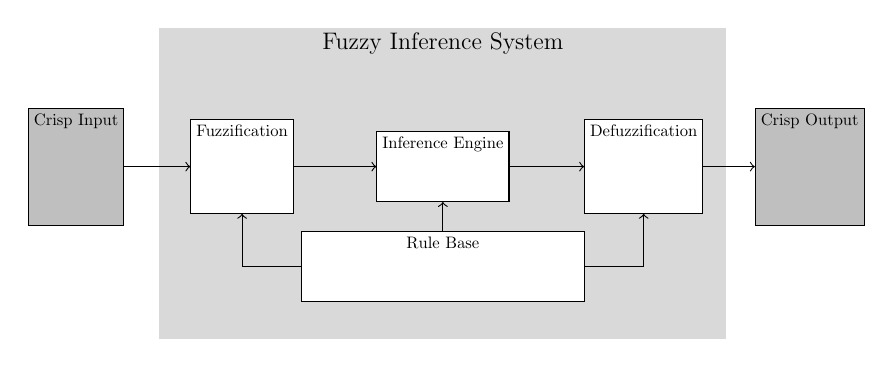
\begin{tikzpicture}[scale=0.6, transform shape]
    \node[fill=gray!30,text depth = 6cm,minimum width=12cm,font=\Large] (main){Fuzzy Inference System};
    \node[draw,fill=white!30, text depth=1cm] at ([yshift=1em]main.center)(infer){Inference Engine};
    \node[draw,fill=white!30, text depth=1cm, minimum width=6cm] at ([yshift=-5em]main.center)(rb){Rule Base};
    \node[draw,fill=white!30, text depth=1.5cm] at ([xshift=5em, yshift=1em]main.west)(fuzz){Fuzzification};
    \node[draw,fill=white!30, text depth=1.5cm] at ([xshift=-5em, yshift=1em]main.east)(defuzz){Defuzzification};
    \node[draw,fill=gray!50, text depth=2cm] at ([xshift=-5em, yshift=1em]main.west)(inp){Crisp Input};
    \node[draw,fill=gray!50, text depth=2cm] at ([xshift=5em, yshift=1em]main.east)(outp){Crisp Output};

    \node at ([xshift=5em, yshift=-5em]main.west)(ghostleft){};
    \node at ([xshift=-5em, yshift=-5em]main.east)(ghostright){};

    \draw[->](inp.east) -- (fuzz.west);
    \draw[->](fuzz.east) -- (infer.west);
    \draw[->](infer.east) -- (defuzz.west);
    \draw[->](defuzz.east) -- (outp.west);
    \draw[->](rb.north) -- (infer.south);
    \draw[->](rb.west) -- (ghostleft.center) -- (fuzz.south);
    \draw[->](rb.east) -- (ghostright.center) -- (defuzz.south);
\end{tikzpicture}

    \caption{Visual representation of a fuzzy inference system}\label{f:fis_block}
\end{figure}

One limiting constraint of FL systems is manifested in a type of state explosion. As the number of inputs,
specifically the number of input MFs, increases, the number of rules needed to cover every case increases as
the product of the number of MFs across all inputs. There have been numerous approaches to overcome this
problem such as cascading small FISs together\cite{ernest2015genetic}, developing more robust methods to guide
convergence\cite{hansen1997convergence} or using approximate fuzzy rule bases\cite{cordon:01bk}. The approach
taken in this work, however, has been to employ GA techniques to tune the MFs or even learn the entire
knowledge base. The dynamic systems being controlled in this research are adequately small that no special
state reduction was deemed necessary in most cases.

\section{Genetic Algorithms}
Genetic algorithms are an evolutionary computing strategy used in optimization and search problems. GAs have
been used in many search and optimization problems\cite{bodenhofer1997ten}. Their effectiveness comes
from the combined ability to explore and exploit. The exploration of of even large search spaces is made
possible with large populations of candidate solutions which are stochastically sampled across the whole
space. Candidates are ranked according to a fitness function and recombined together to create the next
generation. The algorithms exploits learnings in the selection process, favoring recombination of candidates
which ranked well according to the fitness function. In order to maintain gene pool diversity, random mutation
is introduced into each generation as it is created. This process is illustrated in \cref{f:ga_block}. Due to
te stochastic nature of the algorithm, it is not guaranteed to provide an optimal solution and may converge on
a local optimum, but careful selection of hyper parameters such as population size, mutation rates,
recombination methods, and random candidate injection can circumvent these deficiencies somewhat. As the goal
of a GA is to maximize some defintion of a reward, they are commonly employed in reinforcement learning
applications\cite{salimans2017evolution}.

\begin{figure}[ht]
    \centering
    \begin{tikzpicture}[node distance=1cm and 3cm, auto, scale = 0.9, transform shape]
\node[draw, block] (init){initialize $P(t=0)$};
\node[draw, block, below= of init](eval){evaluate $P(t)$};
\node[draw, block, below= of eval](select){select parents from $P(t)$};
\node[draw, block, below= of select](cross){crossover parents into offspring};
\node[draw, block, below= of cross](mut){mutate offspring};
\node[draw, block, below= of mut](ass){form $P(t+1)$ with new offspring};
\node[draw, block, below= of ass](iter){$t=t+1$};
\node[draw, decision, right= of iter](term){met\\termination criteria?};
\node[draw, block, right= of term](fin){finished};

\node [right= of eval](dummy1){};

\draw[line](init) -- (eval);
\draw[line](eval) -- (select);
\draw[line](select) -- (cross);
\draw[line](cross) -- (mut);
\draw[line](mut) -- (ass);
\draw[line](ass) -- (iter);
\draw[line](iter) -- (term);
\draw[line](term) -- (fin);
\draw[line](term.north) -- (dummy1.center) -- (eval);
\end{tikzpicture}

    \caption{Block diagram describing genetic algorithm}\label{f:ga_block}
\end{figure}

Since the fitness function is the sole driver of the algorithm and the solution it provides, great care must
be taken in formulating a fitness function. In robotics applications in particular, formulating a fitness which
adequately encapsulates complex outcomes can be a difficult task\cite{divband2015effect}. This issue will be
revisited a number of times throughout the course of this work.

Another major consideration when utilizing a GA is how to represent or encode a candidate solution for
optimzation. A particularly simple method is to use a binary encoded format\cite{cordon:01bk}, but this
increases the distance between the candidate in its usefule form (phenotype) and its encoded form (genotype)
for many real-values problems\cite{chakraborty1991chromosomal}. A genetic encoding of a FIS is an inherently
heterogenous structure with real values describing the MFs and discrete classes describing the RB. The genetic
operator chosen for a specific genotype will depend on its representation; ideally, the mapping between
genotype and phenotype will be one-to-one such that the combination of two genes will produce a candidate
which performs similarly two its parents. This allows the GA to properly exploit its inherent learning and
converge on a solution.

\subsection{Genetic Operators}
The GA advances by applying operations to the chromosome candidates in its population. The genetic operations
employed in this work are crossover,  mutation, and randomization. Crossover is the operation which allows the
genes from two chromosomes to mix and create new children. If the chromosomes are binary encoded or discrete
valued, the crossover method is generally single-, double-, or n-point crossover. This involves randomly
selecting a point in the encoding string to ``cut'' the chromosomes and swap the tails for single-point, or
sections for n-point.  \Cref{f:dp_cx} demonstrates this process. 



\begin{figure}[ht]
    \centering
    \begin{tikzpicture}[node distance = 0pt]
    \node[dad](d0){0};
    \node[dad, right of=d0](d1){1};
    \node[dad, right of=d1](d2){0};
    \node[dad, right of=d2](d3){1};
    \node[dad, right of=d3](d4){1};
    \node[dad, right of=d4](d5){0};
    \node[dad, right of=d5](d6){1};
    \node[dad, right of=d6](d7){0};
    \node[dad, right of=d7](d8){0};
    \node[mom, below of = d0](m0){1};
    \node[mom, right of=m0](m1){1};
    \node[mom, right of=m1](m2){0};
    \node[mom, right of=m2](m3){0};
    \node[mom, right of=m3](m4){1};
    \node[mom, right of=m4](m5){0};
    \node[mom, right of=m5](m6){0};
    \node[mom, right of=m6](m7){1};
    \node[mom, right of=m7](m8){1};
    \node[left =of d0] {$P^1$:};
    \node[left =of m0] {$P^2$:};

    \node[dad, below of=d0, yshift=-1.5cm](c0){0};
    \node[dad, right of=c0](c1){1};
    \node[dad, right of=c1](c2){0};
    \node[mom, right of=c2](c3){0};
    \node[mom, right of=c3](c4){1};
    \node[mom, right of=c4](c5){0};
    \node[dad, right of=c5](c6){1};
    \node[dad, right of=c6](c7){0};
    \node[dad, right of=c7](c8){0};
    \node[mom, below of = c0](b0){1};
    \node[mom, right of=b0](b1){1};
    \node[mom, right of=b1](b2){0};
    \node[dad, right of=b2](b3){1};
    \node[dad, right of=b3](b4){1};
    \node[dad, right of=b4](b5){0};
    \node[mom, right of=b5](b6){0};
    \node[mom, right of=b6](b7){1};
    \node[mom, right of=b7](b8){1};
    \node[left =of c0] {$C^1$:};
    \node[left =of b0] {$C^2$:};

    \draw[line](m4) -- (c4);
\end{tikzpicture}

    \caption{Double point crossover for binary or discrete valued chromosome.}\label{f:dp_cx}
\end{figure}

For real-values chromosome strings, the crossover methods can be much more complex and more closely related to
solution space. Throughout this work variations on flat crossover will be employed as the main crossover
operation for real-valued portions of the chromosomes\cite{cordon:01bk}. Using this method, a new gene is
created from its parents by drawing a real value from the interval between the parent genes using a uniform
distribution. In many situations, it becomes simpler to write code which always produces two children from a
pair of parents; in these cases, the other gene from a parent interval is selected to be the complement of the
first. Given parents, $P^1 = \left\{p_1^1, p_2^1, \dots, p_n^1\right\},\,P^2=\left\{p_1^2,p_2^2, \dots,
p_n^2\right\}$, children
$C^1=\left\{c_1^1, c_2^1, \dots, c_n^1\right\},\,C^2=\left\{c_1^2,c_2^2,\dots,c_n^2\right\}$ are
created such that:

\begin{align}
    c_i^1 &= \lambda p_i^{min} + (1 - \lambda)p_i^{max}\label{e:flat_cx_c1}\\
    c_i^2 &= (1-\lambda)p_i^{min} + \lambda p_i^{max}\label{e:flat_cx_c2}
\end{align}
where $p_i^{max}=\max(p_i^1,p_i^2)$ and $p_i^{min}=\min(p_i^1,p_i^2)$. An extension, \emph{BLX-$\alpha$}
crossover, is used to expand the selection region beyond the interval between the parents to allow the
crossover function to be more exploratory\cite{cordon:01bk}. This method is described in more detail in
\cref{c:acc}.

Mutation for discrete-valued chromosomes consists of randomly choosing a value from the set of possible values
for a number of genes in achromosome. For this work, mutation is applied to the chromosomes after crossover is
applied. The number of genes in each chromosome to mutate is defined as a hyperparameter. Mutation for
real-valued chromosomes is done with a non-uniform mutation rate which decreases as the generations progress.
This process is detailed in \cref{c:acc}.

For each new generation of chromosomes, a small number of the best performers are preserved untouched from the
previous generation to allow the best genetic material to survive. These chromosomes are called elite. All
chromosomes are ranked according to their fitness to the task and used in crossover proportional to their
fitness. In other words, parents are selected for mutation by drawing chromosomes from the ranked list of
chromosomes using a triangular distribution. \Cref{f:sort-select} shows a distribution laid on top of a sorted
population from which parents would be selected for  recombination. Parents are replaced after selection so
that they may reproduce many times in one generation.

\begin{figure}
    \centering
    \begin{tikzpicture}
    \draw[fill=red!30, draw=none](-6.2,-1) -- (6.2,-4) -- (-6.2,-4) -- cycle;
    \node(presort){
            \begin{minipage}{0.9\textwidth}
                \begin{align*}
                    &P^{0}&&P^{1}&&P^{2}&&P^{3}&&P^{4}&&P^{5}&&P^{6}&&P^{7}\\
                    &0.63&&0.67&&0.89&&0.60&&0.43&&0.26&&0.82&&0.03
                \end{align*}
            \end{minipage}
        };
    \node[below of= presort, yshift=-3.5cm] (sorted){
            \begin{minipage}{0.9\textwidth}
                \begin{align*}
                    &P^{7}&&P^{5}&&P^{4}&&P^{3}&&P^{0}&&P^{1}&&P^{6}&&P^{2}\\
                    &0.03&&0.26&&0.43&&0.60&&0.63&&0.67&&0.82&&0.89
                \end{align*}
            \end{minipage}
        };
    \draw[line](0,-1) -- (0,-2);

\end{tikzpicture}




    \caption{Population sorting and selection distribution overlay}\label{f:sort-select}
\end{figure}
    
\section{Genetic Fuzzy Systems}
Genetic Fuzzy Systems (GFS) here describe FL systems which have been tuned or learned using GA strategies.
Tuning a GFS implies that the rule base is static, while the GA is allowed to operate on only the MF values or
input/output scaling. Learning, on the other hand, implies that the RB itself is allowed to vary. For this
research, except where otherwise stated, GFSs are allowed to learn the RB from scratch. In order to
effectively use GAs to interact with FISs, some simplifying constraints are commonly imposed on the GFS to
ease the use of genetic operators. One such constraint that is frequently used in this research is to mandate
strict triangular or trapezoidal MFs. This allows the entire collection of MFs across all of the inputs to be
described by either 3- or 4-tuples of sorted real values. As the GA is allowed to operate on the MFs, checks
are placed to make sure that like MFs are combined in recombination and that the children contain valid MFs.
All of this is eased by constraining a GFS to only contain triangular or trapezoidal MFs. Additionally, it is
assumed that the RB completely covers the input combination possibilities. This is similar to a fully
connected layer of neurons in a NN. This forces the number of rules to be equal to the product of the number
of MFs across all inputs; as a result of this constraint, the number of rules can quickly explode as inputs
are added to the system or inputs are granularized with additional MFs. To prevent RB explosion, FISs in this
work are kept minimal. Knowing the numpber of MFs, the RB can be reduced to a single string of integers, where
each integer is equal to the index of one of the output MFs. Thus is in way, we can fully describe a FIS with
one heterogenous string of values. For instance, the FIS illustrated in \crefrange{f:fuzzysets}{f:outputfan}
with the RB in \cref{t:fanspeed} would be described completely by the list:

\begin{equation*}
    \left(0, 0, 55, 65\right) \left(55, 65, 75\right) \left(65, 75, 100, 100\right)
    |\left(0, 0, 0.25\right) \left(0, 0.25, 1\right) \left(0.25, 1, 1\right)
    \left[0, 1, 2\right]
\end{equation*}
where each MF tuple is grouped in $\left(\right)$, input is separated from output with $|$, and the RB is in
$\left[\right]$. The genetic operations on MF paramaters are any operations which can work with real values,
and the RB is constrained to n-point crossover.

\section{Motivation and Problem Statement}
This work explores the utility of using the GFS approach to exert control on dynamic systems. Because of the
ability of a GFS to deal with imprecision and uncertainty, it can be an adaptive controller which can respond
to changes in plant dynamics. Also, if the GFS is kept small, the trained system can be interpreted by a human
operator with linguistic rules. With the rise in popularity of black box decision-making frameworks in recent
years, interpretability has become a topic of fervent
research\cite{ribeiro2016should,lipton2016mythos,zeiler2014visualizing,dong2017improving}. Learning [rovides
the benefit of exhibiting emergent behavior, but usually at the cost of interpretability. Genetic fuzzy
systems may provide a middle ground; starting with a hand-crafted template, and then allowing a GA to learn
behavior, the final model can still be assigned lingistic variables and given meaning. 

This thesis is composed of a handful of problems which were approached using a GFS.
\begin{enumerate}
    \item {\bf Two-cart flexible system}. First, the problem of controlling a two-cart system is addressed.
        The system is allowed to move freely along a track with the objective of meeting, but not exceeding, a
        goal. This system exhibits two modes of behavior: over large distances, it behaves similar to a rigid
        structure; when finer control is needed in the terminal phase, the flexible body vibrations dominate
        the behavior. A controller is tuned to handle this system in \cref{c:acc}.

    \item {\bf F-4 Phantom Pitch Controller}. Secondly, a pitch attitude controller for the F-4 fighter jet is
        designed. This system is allowed to train on only a nominal flight condition, but then subjected to
        large degradations in plant dynamics and evaluated. The performance is shown to exceed that of a PID
        controller in \cref{c:f4}.

    \item {\bf sUAS Precision Landing} Finally, a controller for a small quadrotor is designed to guide the
        vehicle to a moving target using only visual feedback from an on-board camera. This problem is
        constrained by physical systems, so simulation environments, controllers, computations, and sensors
        are chosen such that the system will be more readily physically realized. The benefits and
        shortcomings of the Robot Operating System with the Gazebo simulation environment are also discussed
        at length. This discussion comprises \cref{c:landing}.
\end{enumerate}

